\label{subsec:tracks_uncer}

We incorporate dedicated uncertainties related to track reconstruction, particularly for tracks associated with small-R jets, as outlined in the recommendations on \mbox{\texttt{\href{https://twiki.cern.ch/twiki/bin/viewauth/AtlasProtected/QuarkGluonTagging\#Current_Recommendations}{QuarkGluonTagging}}} and \mbox{\texttt{\href{https://twiki.cern.ch/twiki/bin/view/AtlasProtected/TrackingCPRecsRun2Final\#Track_Systematics_Tools}{TrackingCPRecsRun2Final}}}. 
%Specifically, the ghost-associated track multiplicities of our jets are utilized as inputs to the recurrent layer of the final network.

The procedure in \cite{ATL-PHYS-PUB-2017-009} is used to derive these track multiplicity related uncertainties, of which there are five main components:
\begin{itemize}
    \item fake track efficiency: the uncertainty from the track mis-reconstruction rate;
    \item track efficiency: the uncertainty from the track reconstruction efficiency;
    \item experimental: the uncertainty in charged particle multiplicity, derived as in \cite{CERN-PH-EP-2016-001};
    \item PDF: the theory uncertainty from the parton distribution function;
    \item matrix element: the theory uncertainty from the matrix element calculation;
\end{itemize}
The impacts from these uncertainties are expected to be low.

%%%%%%%%%%%%%%%
%%%We take into account some dedicated uncertainties on the tracks' reconstruction, 
%%%in particular, for the tracks associated to the small-R jets 
%%%\mbox{\texttt{\href{https://twiki.cern.ch/twiki/bin/viewauth/AtlasProtected/QuarkGluonTagging\#Current_Recommendations}{QuarkGluonTagging}}}
%%%\mbox{\texttt{\href{https://twiki.cern.ch/twiki/bin/view/AtlasProtected/TrackingCPRecsRun2Final\#Track_Systematics_Tools}{TrackingCPRecsRun2Final}}}
%%%. 
%%%Indeed, we use the track multiplicities of the ghost associated tracks to our jets as input to the recurrent layer of the final network.
%%%
%%%The procedure in ~\cite{ATL-PHYS-PUB-2017-009}
%%%is used to derive these track multiplicity related uncertainties,
%%%of which there are five main components:
%%%\begin{itemize}
%%%    \item fake track efficiency: uncertainty from track mis-reconstruction rate;
%%%    \item track efficiency: uncertainty from track reconstruction efficiency;
%%%    \item experimental: uncertainty in charged particle multiplicity, derived as in ~\cite{CERN-PH-EP-2016-001};
%%%    \item PDF: theory uncertainty from parton distribution function;
%%%    \item matrix element: theory uncertainty from matrix element calculation;
%%%\end{itemize}
%%%Figures~\ref{fig:1lep_TrackUncCR}, \ref{fig:1lep_TrackUncSR} shows the variations from these sources of
%%%track multiplicity uncertainties for background and signal events in the \olep signal regions.
%%%The impacts from these uncertainties are expected to be low, as they are less than 5\% in the high RNN
%%%bins.

%%%\begin{figure}[ht]
%%%    \centering
%%%        \subfigure[Merged HP SR \ttbar]{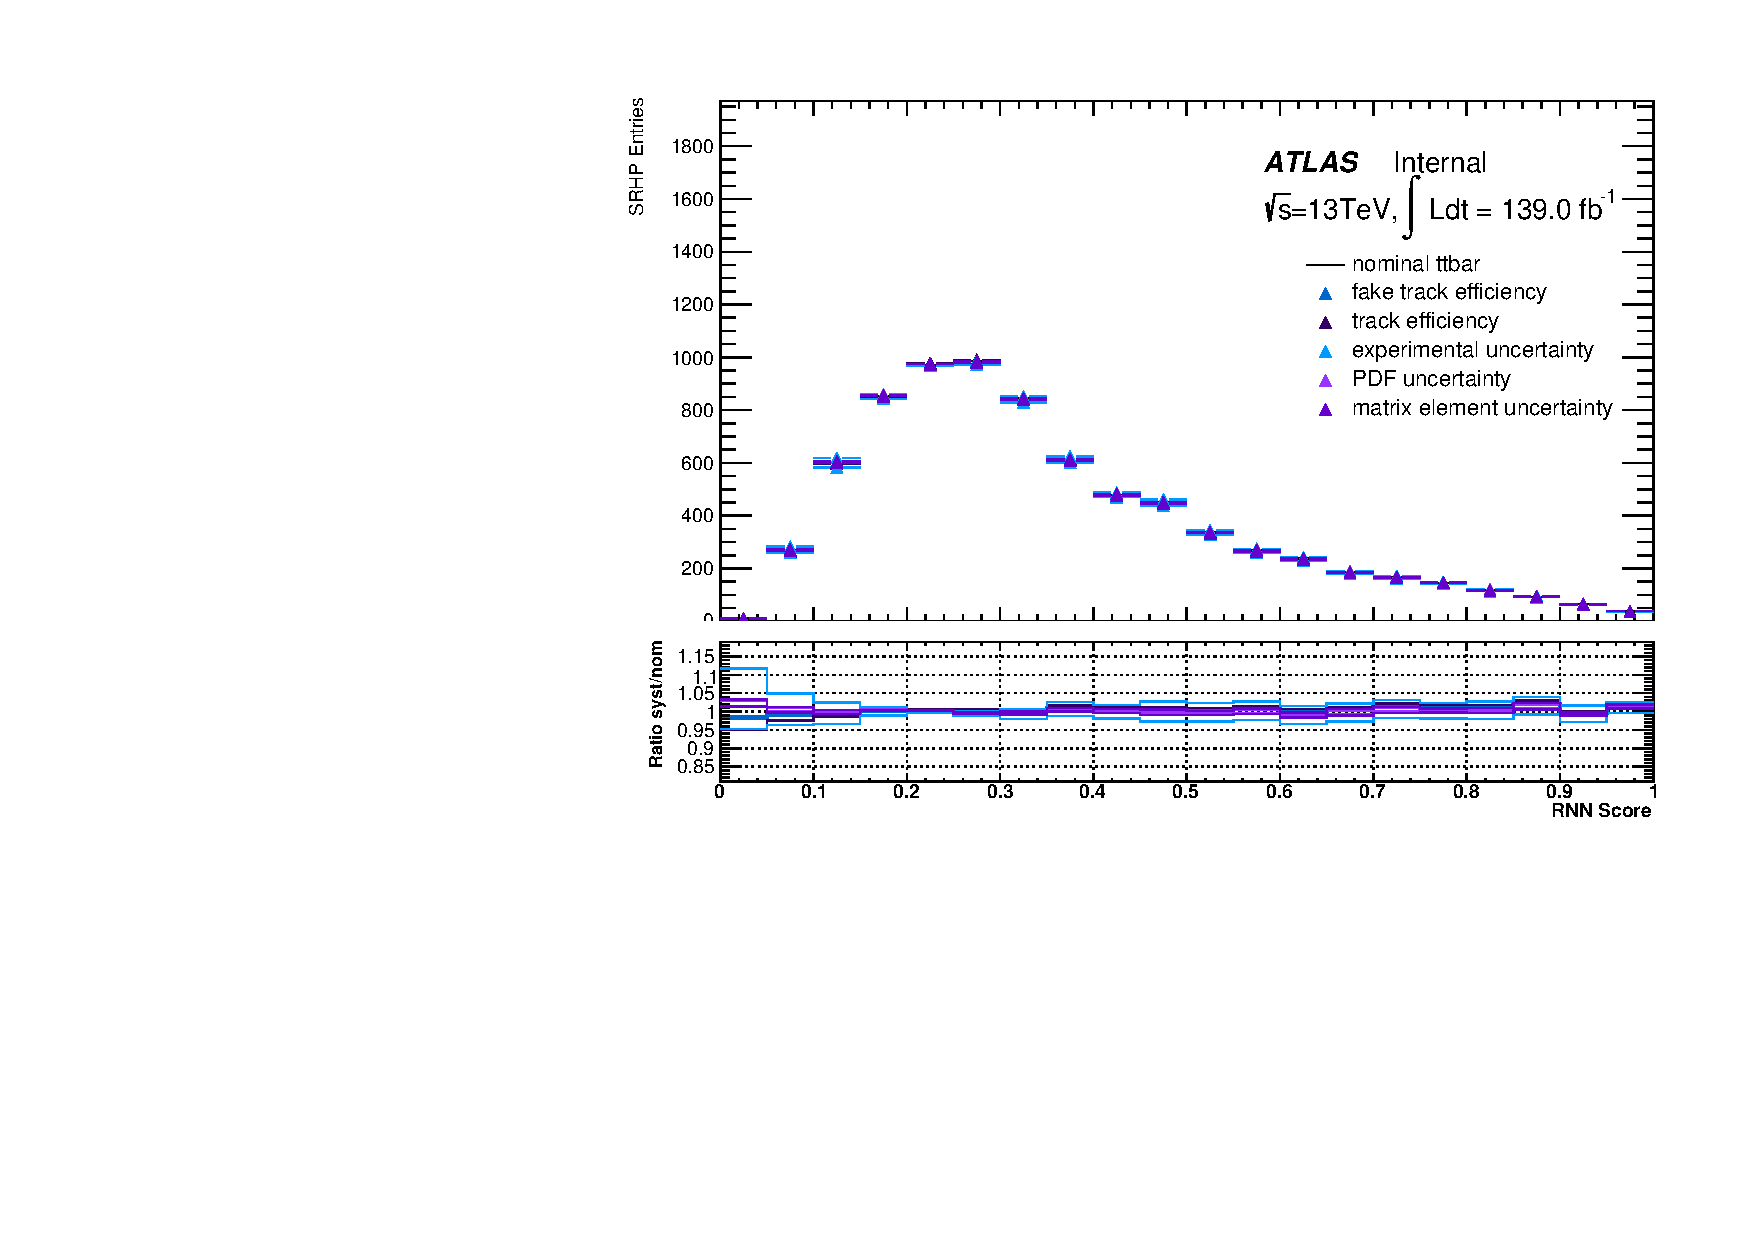
\includegraphics[width=0.45\textwidth]{figures/1lep/TrackSyst/SystQGSRHP_ttbar_RNN.pdf}}
%%%        \subfigure[Merged HP SR W]{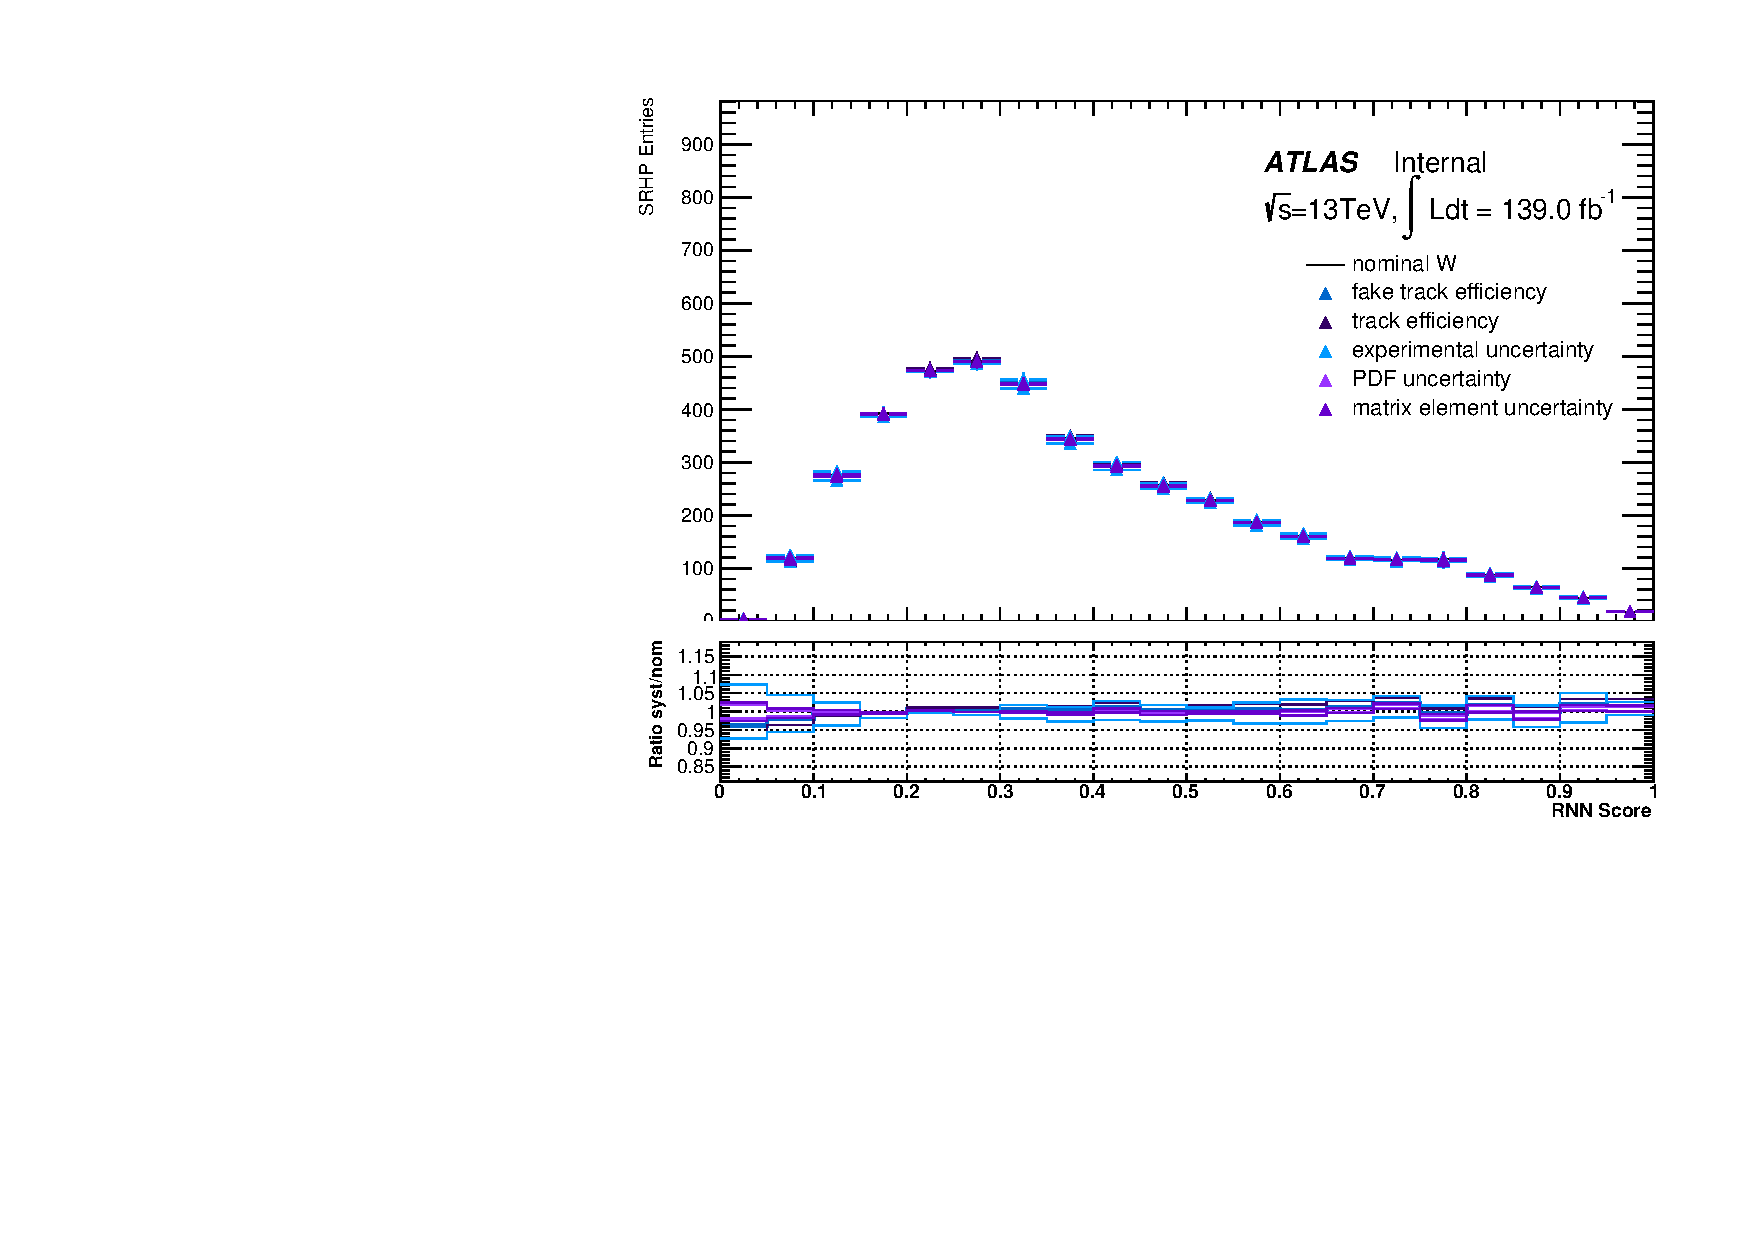
\includegraphics[width=0.45\textwidth]{figures/1lep/TrackSyst/SystQGSRHP_W_RNN.pdf}}
%%%        \subfigure[Merged LP SR \ttbar]{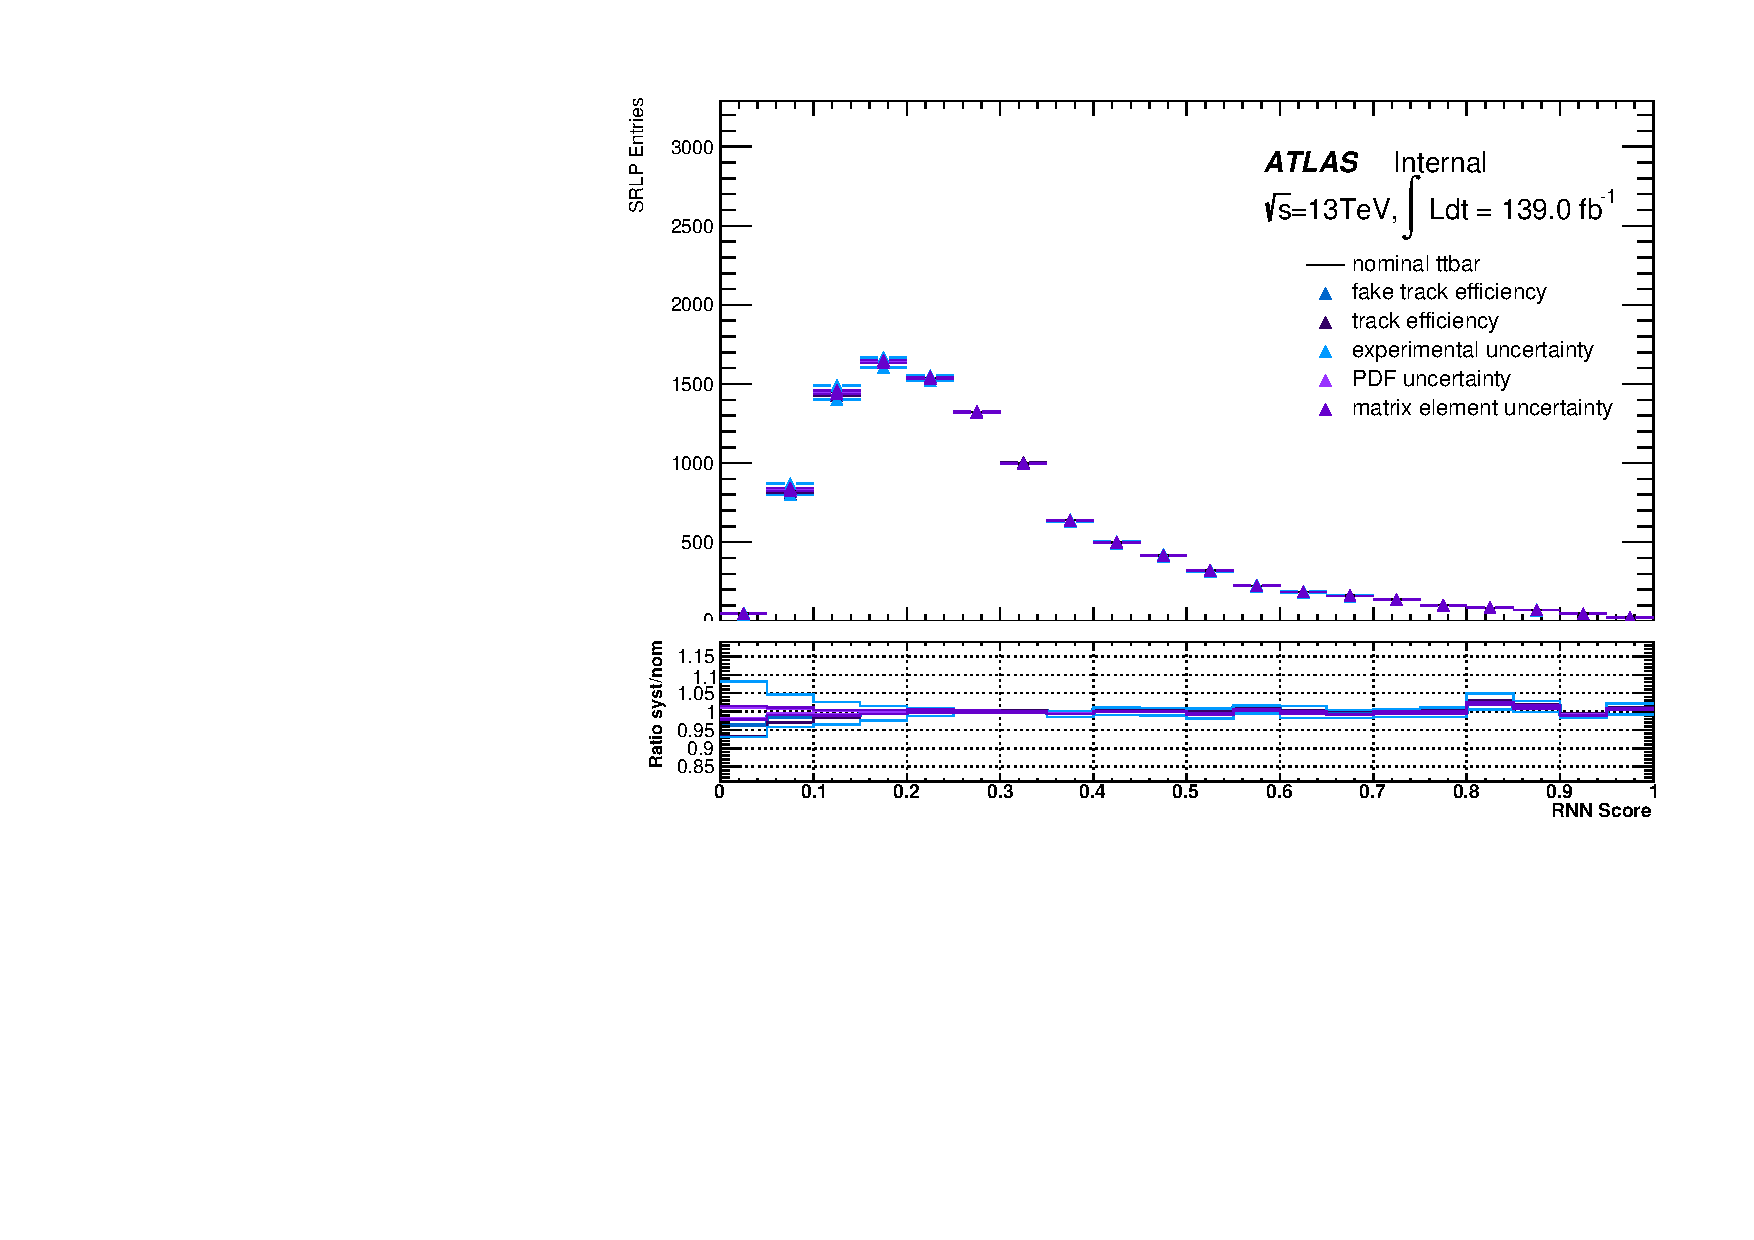
\includegraphics[width=0.45\textwidth]{figures/1lep/TrackSyst/SystQGSRLP_ttbar_RNN.pdf}}
%%%        \subfigure[Merged LP SR W]{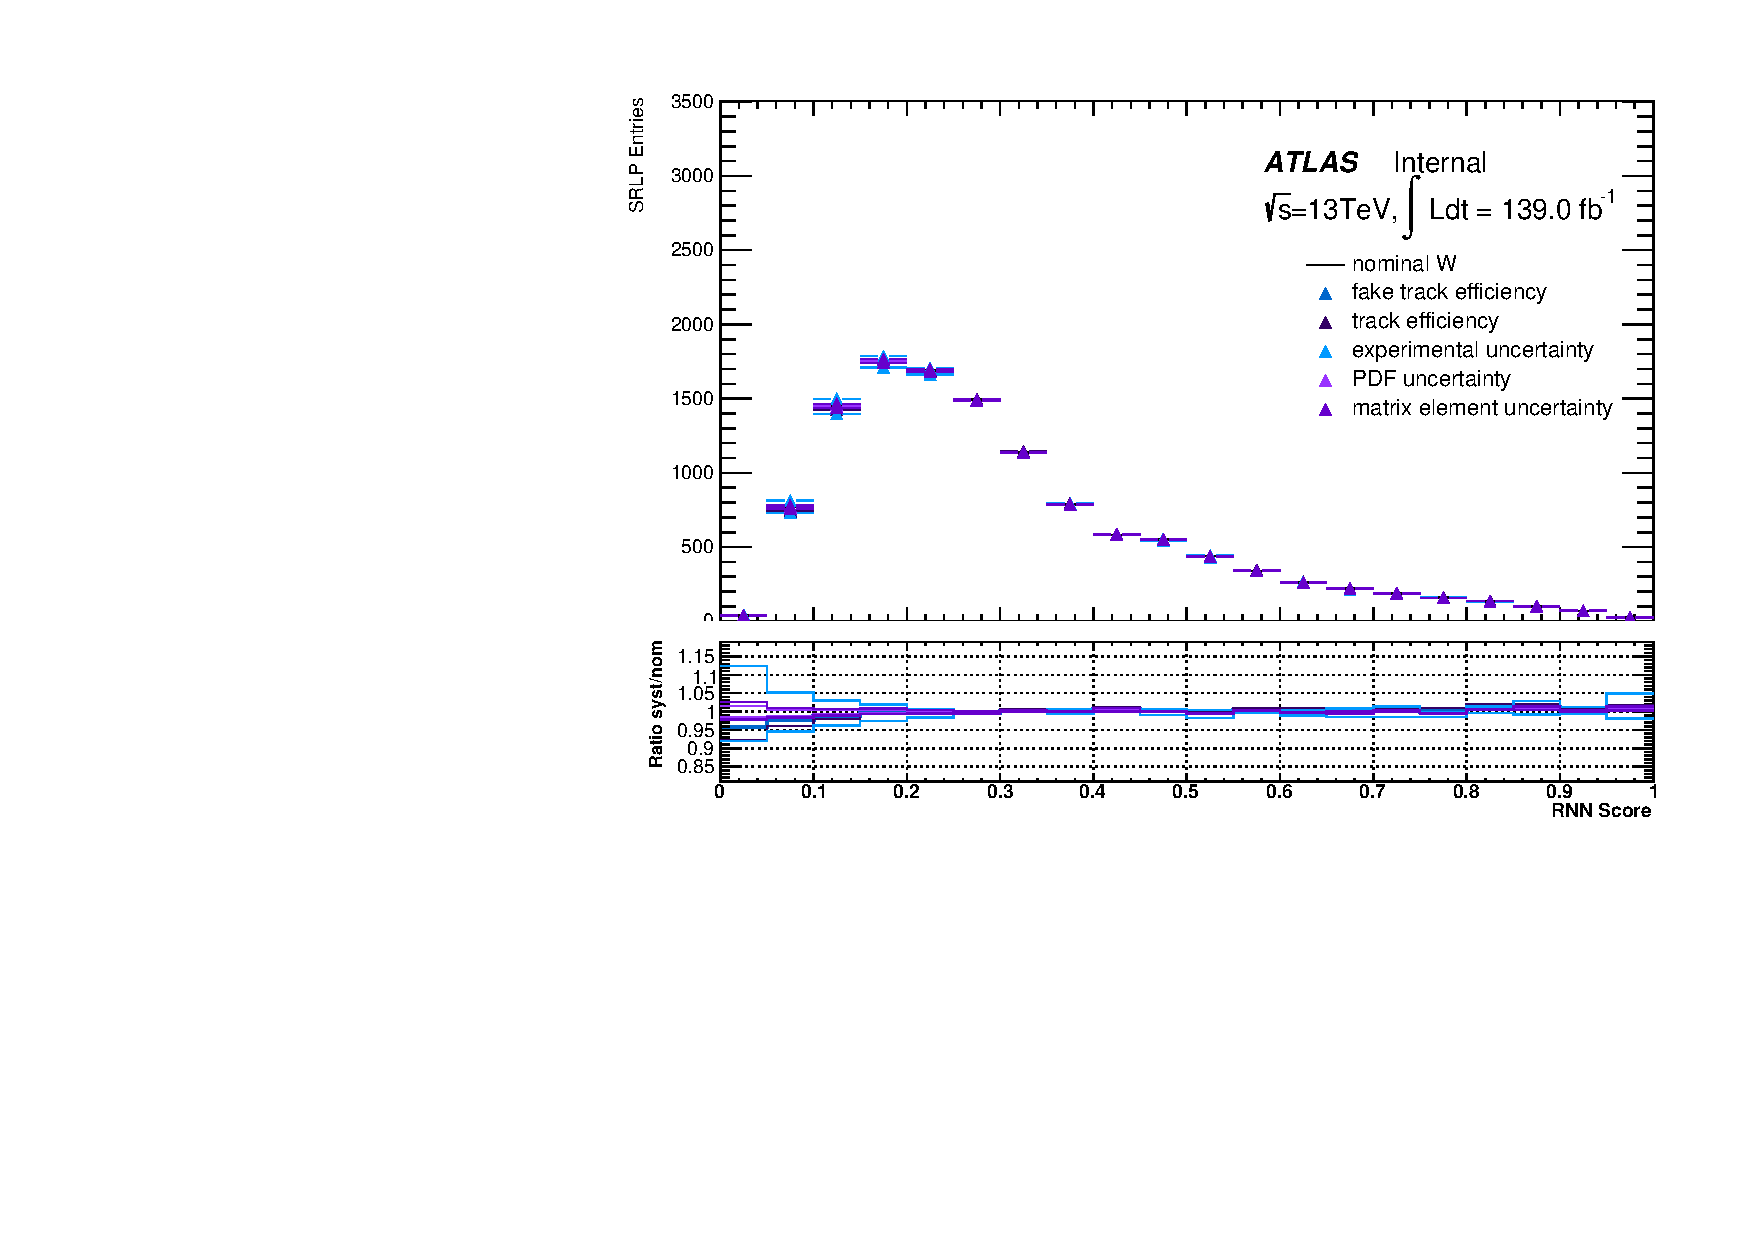
\includegraphics[width=0.45\textwidth]{figures/1lep/TrackSyst/SystQGSRLP_W_RNN.pdf}}
%%%        \subfigure[Resolved SR \ttbar]{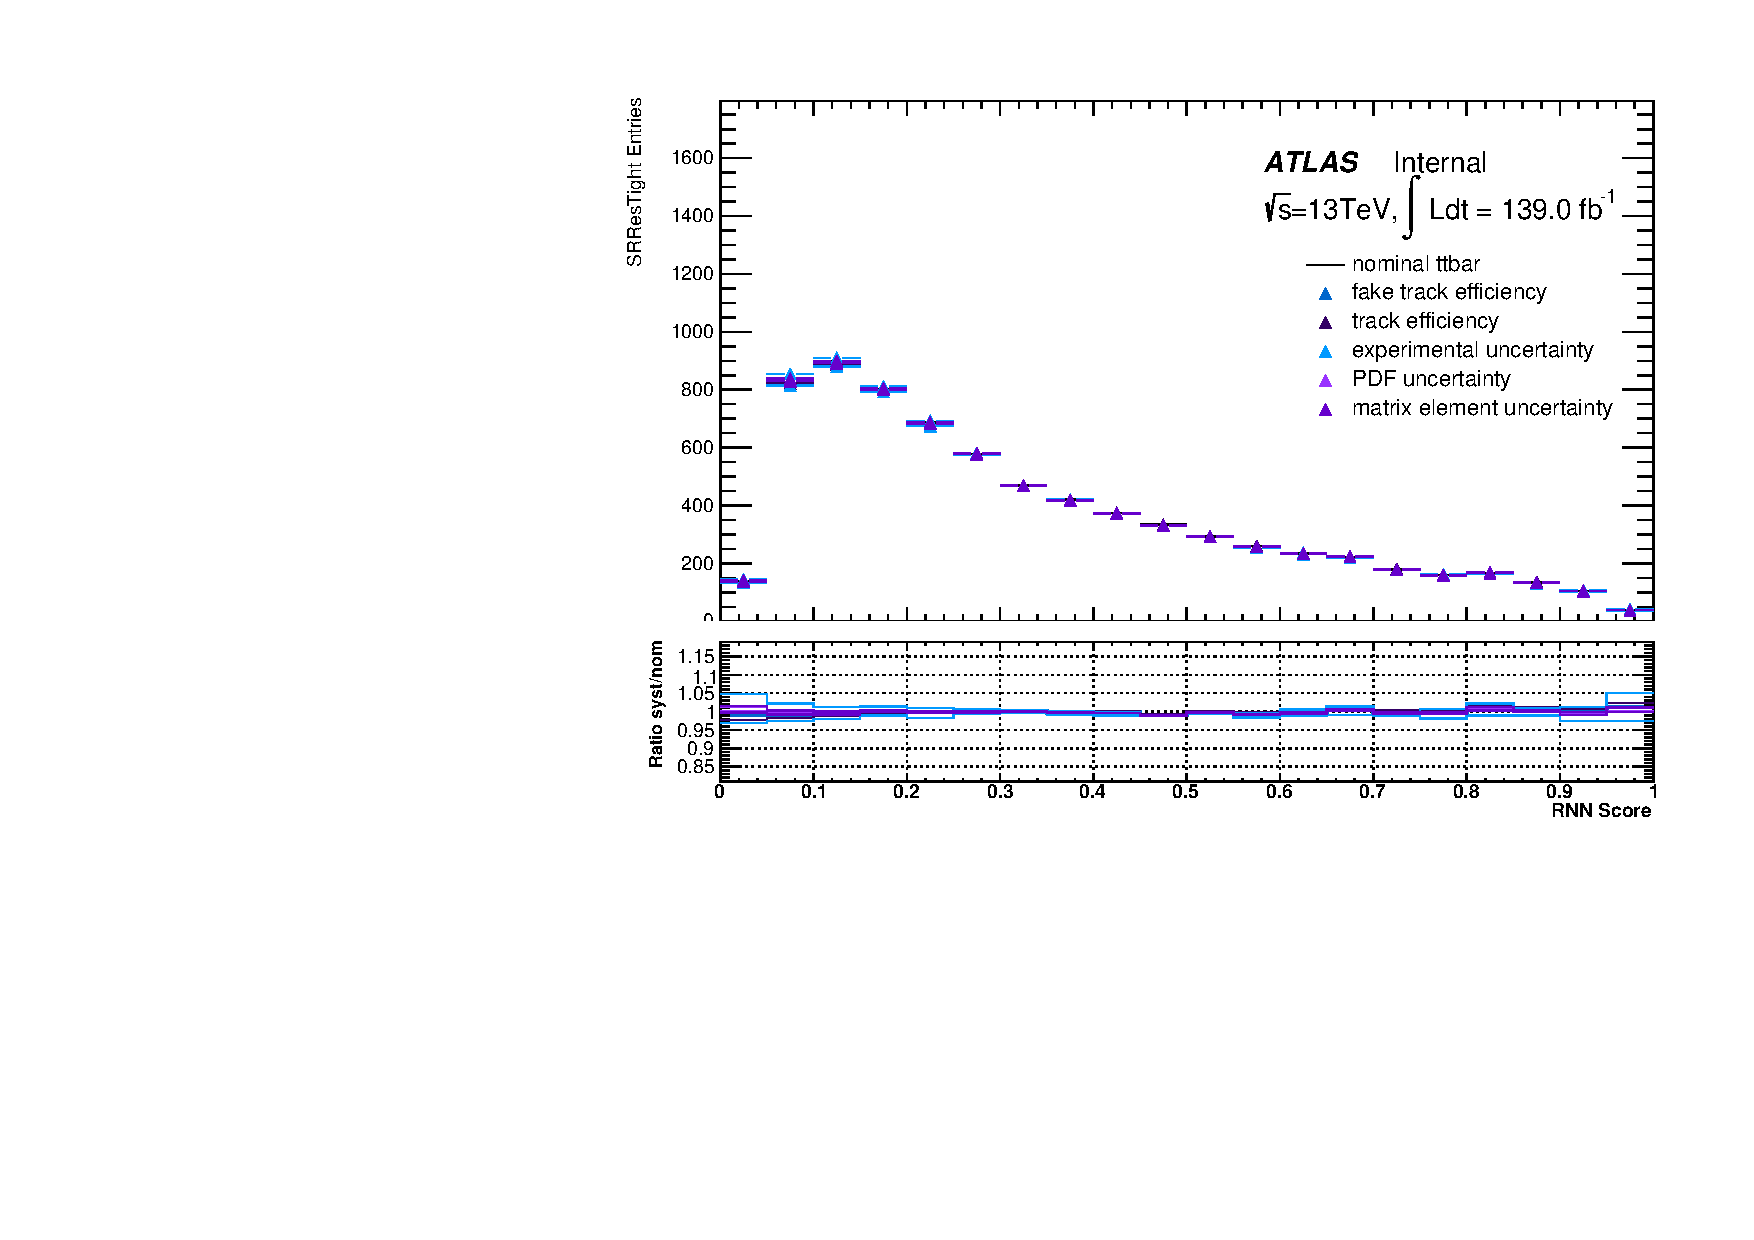
\includegraphics[width=0.45\textwidth]{figures/1lep/TrackSyst/SystQGSRResTight_ttbar_RNN.pdf}}
%%%        \subfigure[Resolved SR W]{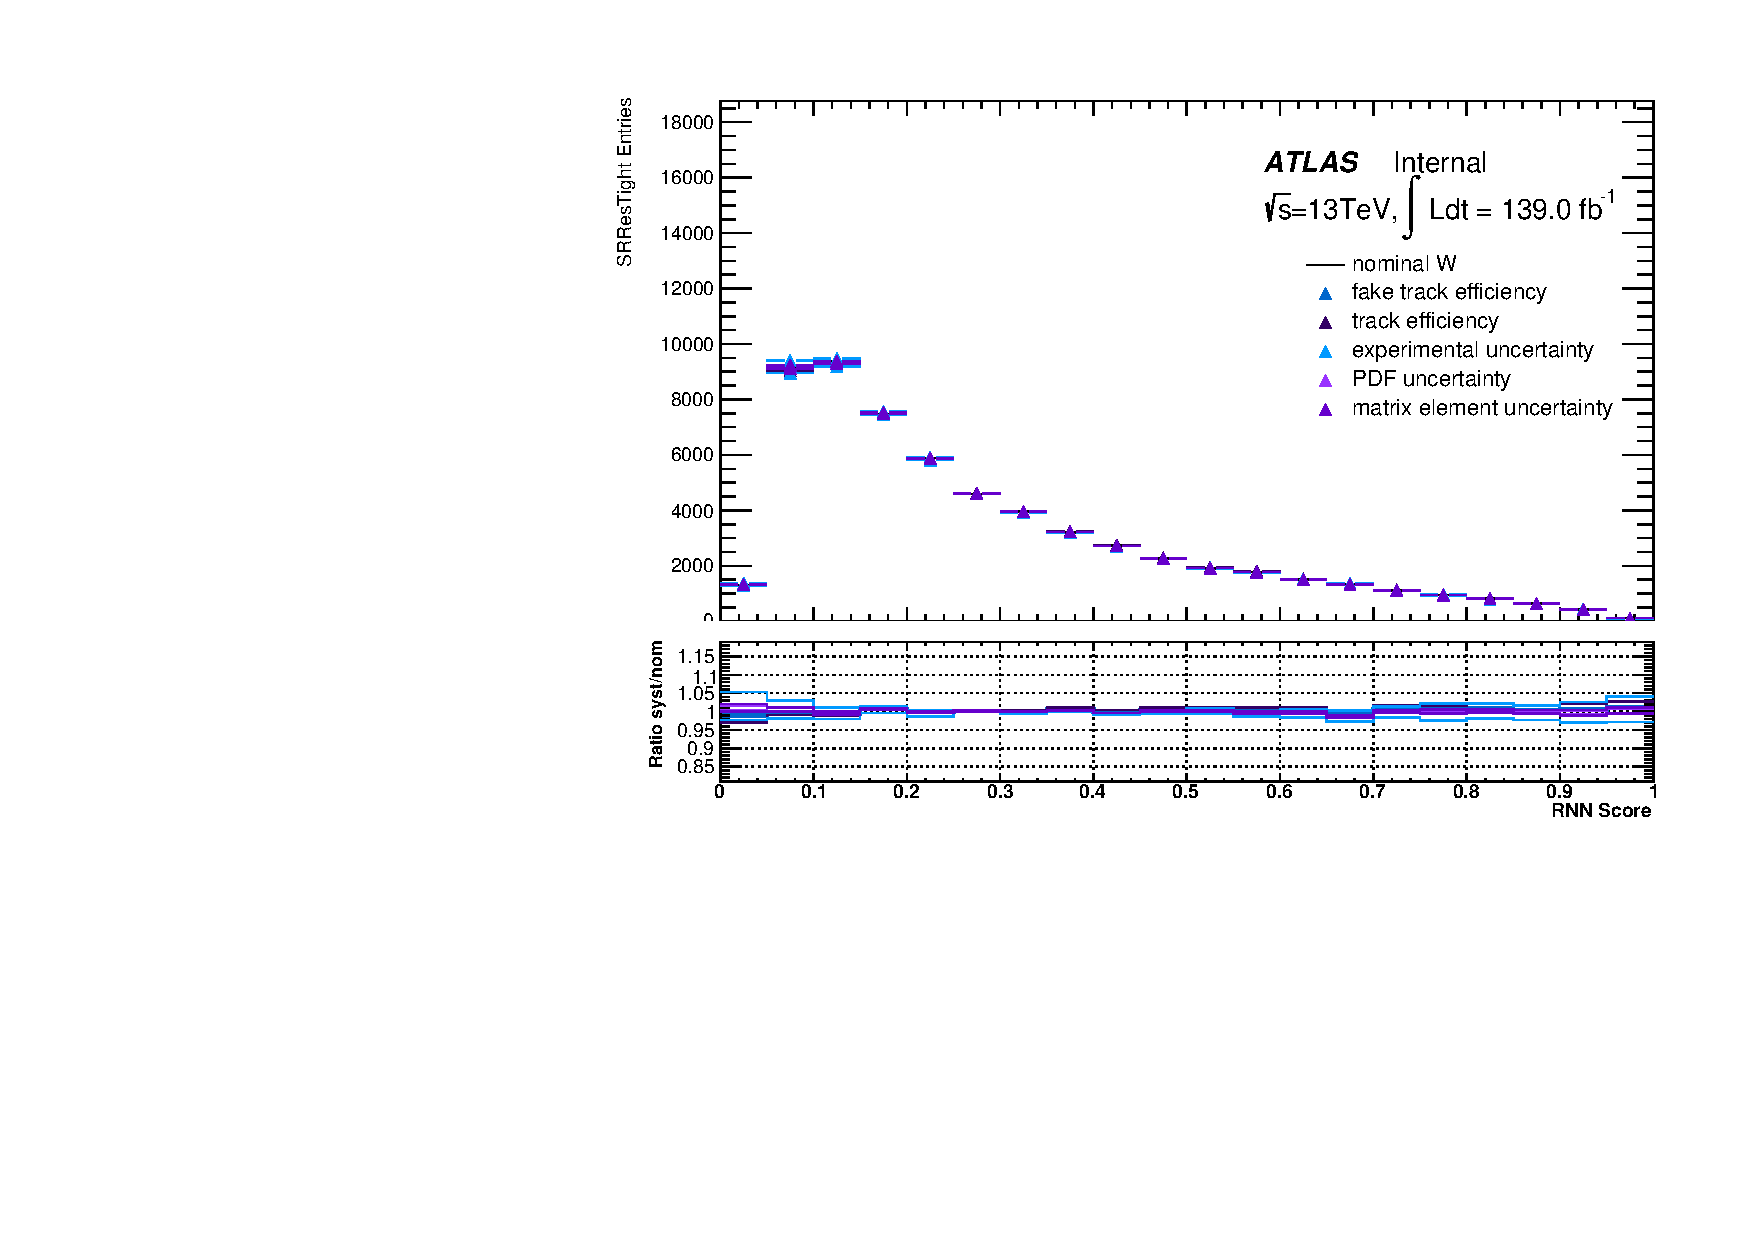
\includegraphics[width=0.45\textwidth]{figures/1lep/TrackSyst/SystQGSRResTight_W_RNN.pdf}}
%%%        \caption{Track multiplicity related uncertainties for \ttbar and \Wjets events in the signal regions. }
%%%    \label{fig:1lep_TrackUncCR}
%%%\end{figure}
%%%
%%%\begin{figure}[ht]
%%%    \centering
%%%        \subfigure[Merged HP SR Signal]{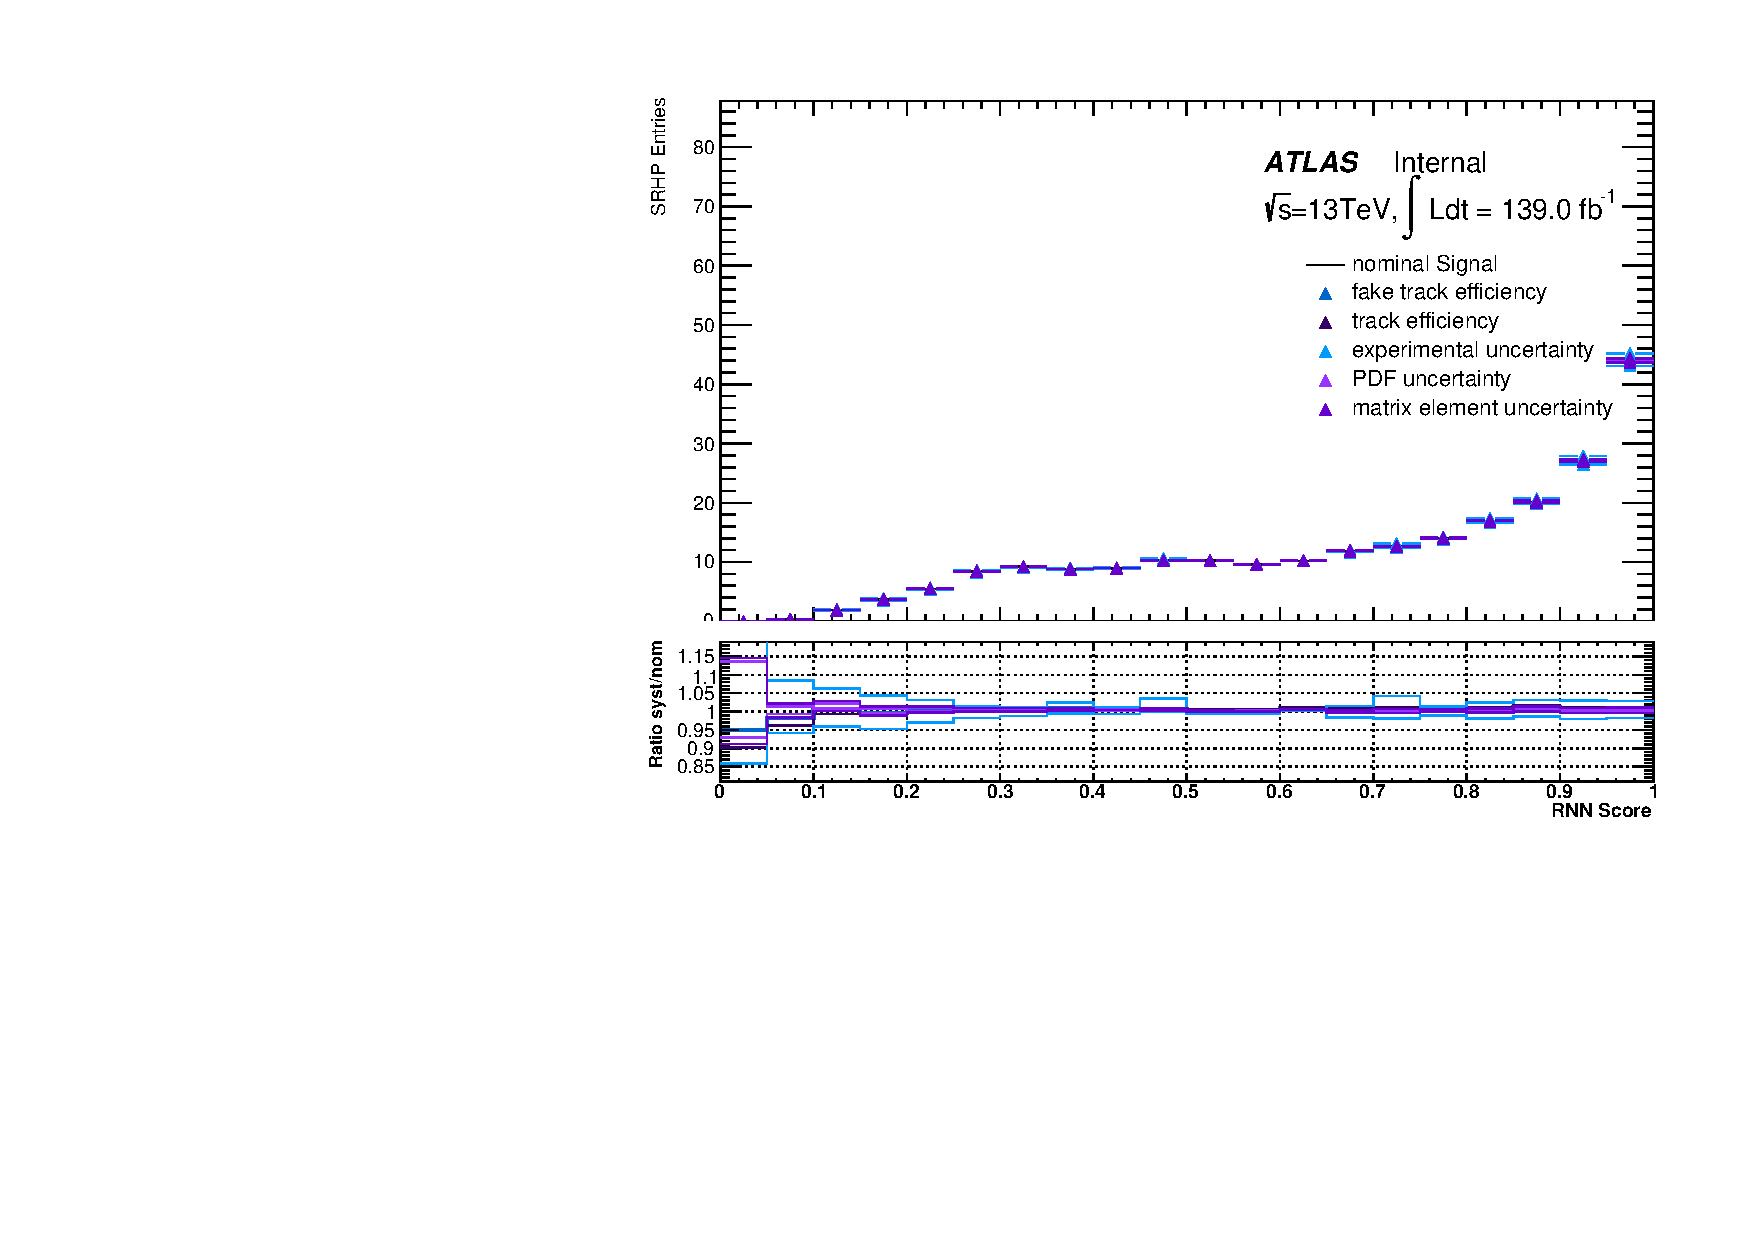
\includegraphics[width=0.45\textwidth]{figures/1lep/TrackSyst/SystQGSRHP_Signal_RNN.pdf}}
%%%        \subfigure[Merged LP SR Signal]{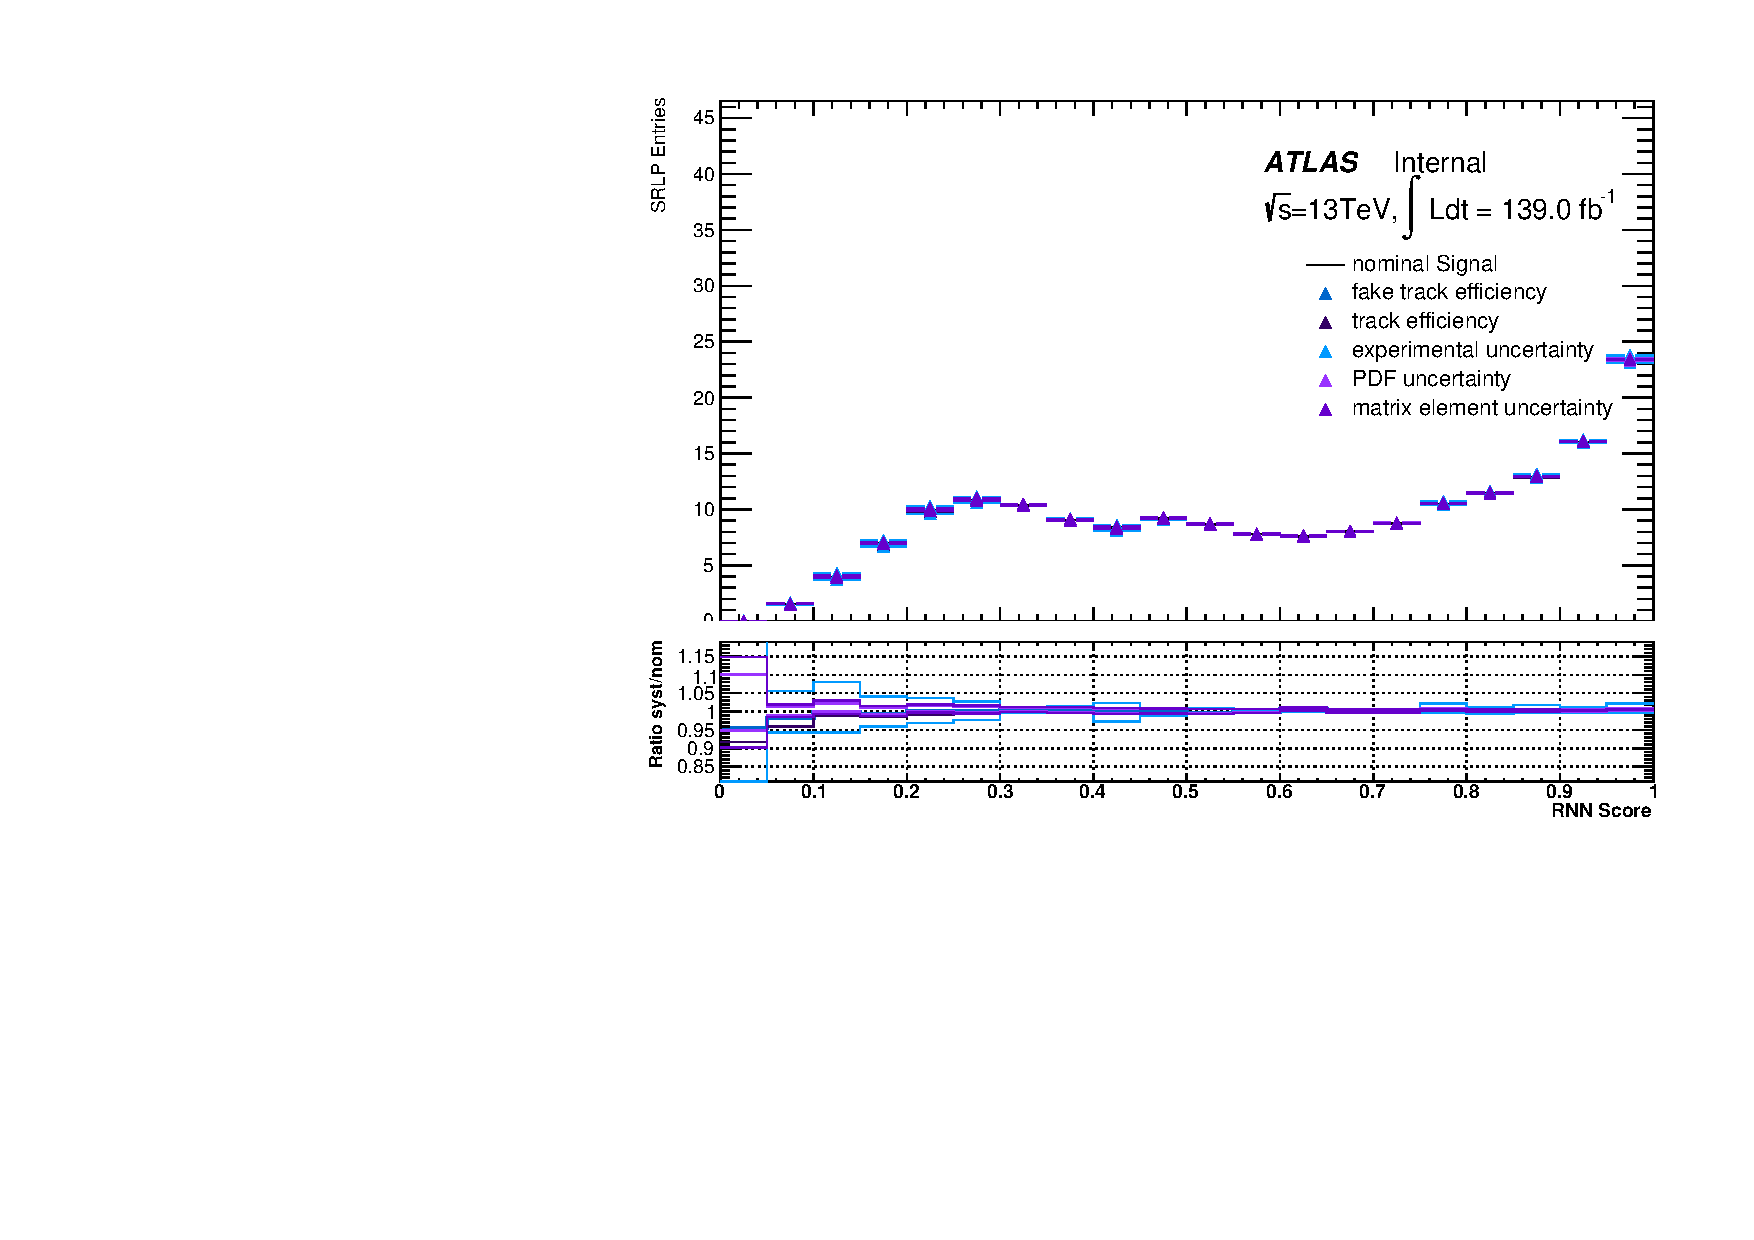
\includegraphics[width=0.45\textwidth]{figures/1lep/TrackSyst/SystQGSRLP_Signal_RNN.pdf}}
%%%        \subfigure[Resolved SR Signal]{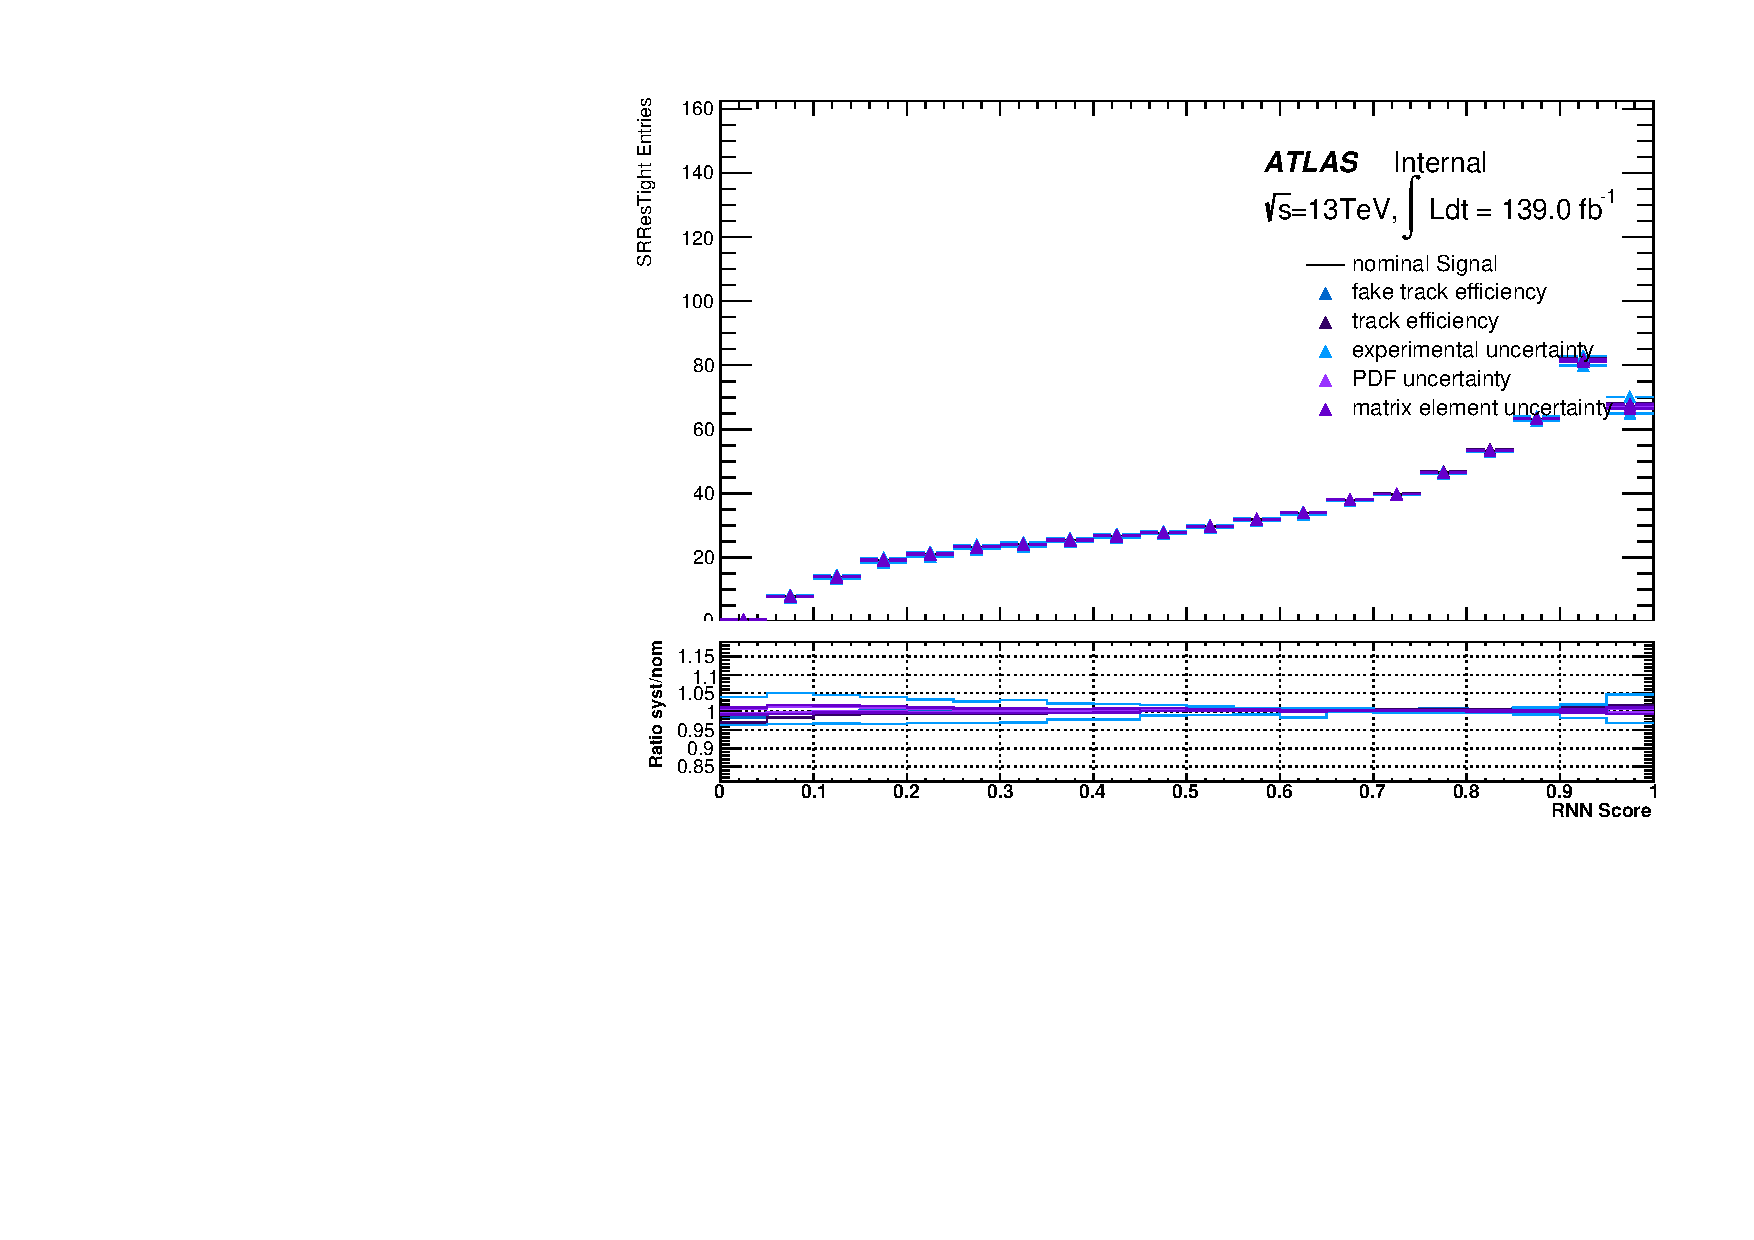
\includegraphics[width=0.45\textwidth]{figures/1lep/TrackSyst/SystQGSRResTight_Signal_RNN.pdf}}
%%%        \caption{Track multiplicity related uncertainties for signal events in the signal regions. }
%%%    \label{fig:1lep_TrackUncSR}
%%%\end{figure}


%both from quick statistics test 
%both from past studies in the VV semi-leptonic resonant search \cite{Bachas:2646593}.
